\chapter{Basistechnologien}
\thispagestyle{standard}
\pagestyle{standard}
\renewcommand{\footrulewidth}{0.4pt}
\lfoot{\small Markus Haas}

\section{Modbus Protokoll}

In diesem Kapitel wird das Modbus Protokoll beschrieben.
Der Protokolladapter ist für Modbus TCP entwickelt worden, deshalb wird auch vorwiegend diese Version erklärt. Entwickelt wurde das Protokoll aber ursprünglich für die serielle Schnittstelle. Daher wird zuerst das Protokoll für die serielle und anschließend die Erweiterung für TCP beschreiben.

\subsection{Geschichte}

Das Modbus Protokoll für die serielle Schnittstelle wurde von der Firma Modicon entwickelt und 1979 veröffentlicht. Der Name der Firma Modicon ist heute Schneider Electric. Mit Modbus TCP/IP wurde von Schneider Electric 1999 ein offener Standard entwickelt, um Modbus auch über Ethernet nutzbar zu machen. Die Rechte an Modbus wurden 2004 an die Modbus Organization übergeben, welche zurzeit das Protokoll betreut \cite{ModbusFAQ}. 


\subsection{Grundlagen}

Modbus ist ein Protokoll, welches sich auf den Schichten 2 und 7 des OSI Schichtmodells befindet. Das Protokoll stellt eine Client-Server Verbindung zwischen den Teilnehmern her. Es funktioniert nach dem Request-Response Prinzip. Die Funktionen des Protokolls werden durch sogenannte Funktionscodes spezifiziert \cite{ModbusSpecification}. 

\begin{figure}[h]
	\centering
	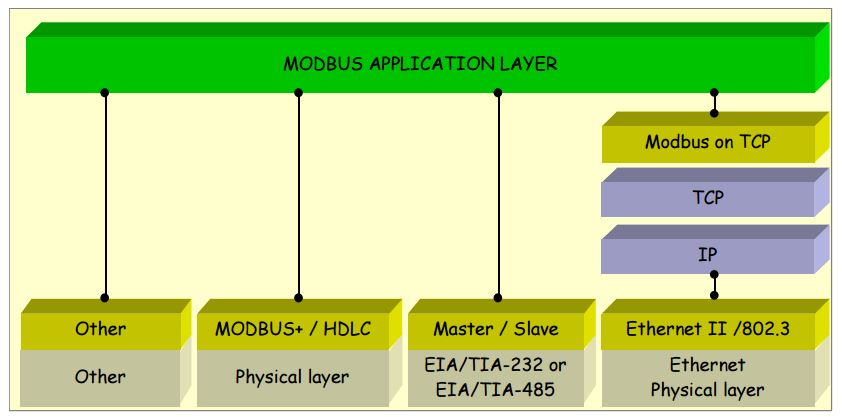
\includegraphics[width=14cm]{BilderAllgemein/ModBusUebersicht.jpg}\medskip
	\caption{Schichten des ModBus Protokolls \cite[S.2]{ModbusSpecification}}
	\label{fig:ModbusSchichten}
\end{figure}

\vspace{1cm} Abbildung \ref{fig:ModbusSchichten} stellt die unterschiedlichen Modbus Varianten dar.


\begin{itemize}
    \item Modbus TCP/IP
    \newline Master/Slave Kommunikation über Ethernet
    \item Modbus RTU
    \newline serielle Master/Slave Kommunikation über RS232 oder RS485
    \item Modbus Plus
	\newline ein Netzwerk mit Tokenweitergabe
\end{itemize}


\subsection{Protokollaufbau}
\label{sec:Protokollaufbau}
Wie aus Abbildung \ref{fig:ModbusFrame} ersichtlich, besteht die \ac{PDU} aus Funktionscode und den Daten. Für den Funktionscode ist ein Byte reserviert. Daraus ergeben sich 256 Funktionscodes, wobei der Bereich 128 - 255 reserviert ist für die Exception Antworten und 0 ein ungültiger Funktionscode ist. Für die Funktionscodes ergibt sich daraus ein nutzbarer Bereich von 1 - 127. Das Modbus Protokoll ist ursprünglich für die serielle Schnittstelle entwickelt worden. Dabei wurde die \ac{ADU} auf 256 Bytes begrenzt. Von den 256 Bytes werden 1 Byte für die Modbus Server Adresse verwendet und 2 Bytes für die \ac{CRC}. Daraus ergibt sich eine Länge von 253 Bytes für die PDU. Weiters lässt sich dadurch für das Datenfeld eine Länge von 252 Bytes berechnen. Modbus verwendet die Big-Endian Byte Reihenfolge für Daten und Adressen \upshape \cite{wilamowski2011industrial}.

\begin{figure}[h]
  	\centering
  	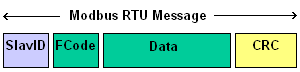
\includegraphics[width=10cm]{BilderAllgemein/ModbusFrame.png}\medskip
	\caption{Schematische Darstellung eines Modbus RTU Frames \cite{ModbusTCPImplementation}} 
 	\label{fig:ModbusFrame}
\end{figure}
\clearpage

Es werden 3 PDUS von Modbus spezifiziert
\begin{itemize}
      \item Modbus request PDU
      \newline Diese wird vom Client generiert und an den Server übermittelt.
      \item Modbus response PDU
     \newline Diese wird vom Server als Antwort an den Client gesendet, wenn die Aktion am Server erfolgreich war.
      \item Modbus exception response PDU
      \newline Diese wird vom Server als Antwort an den Client gesendet, wenn am Server während der Aktion ein Fehler auftrat.
\end{itemize}


Abbildung \ref{fig:FehlerfreieTransaktion} zeigt den Ablauf einer erfolgreichen Modbus Transaktion. Dabei wird durch den Funktionscode und den dazugehörigen Daten ein Request an den Server gesendet. Anschließend wird die PDU mit demselben Funktionscode und den Nutzdaten wieder an den Client gesendet \upshape \cite{ModbusSpecification}.

\begin{figure}[h]
 	\centering
 	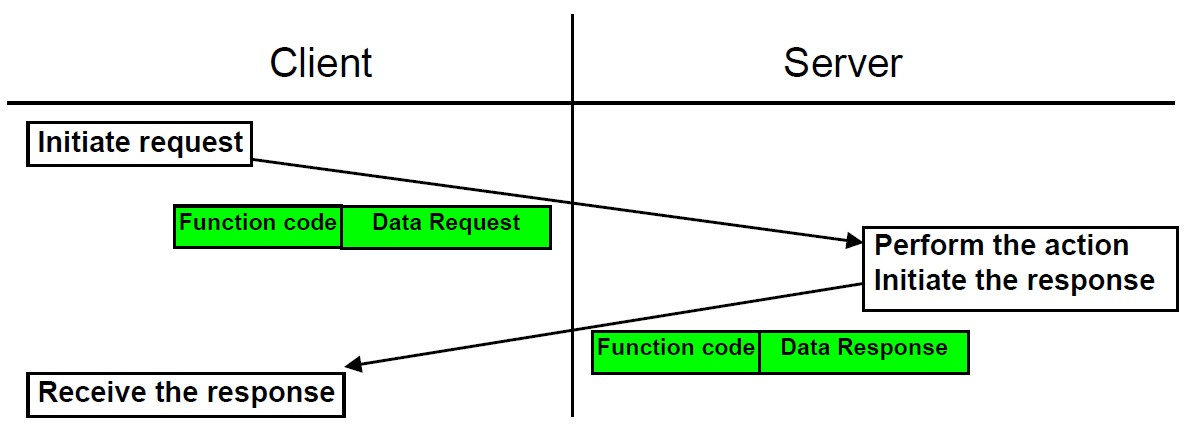
\includegraphics[width=14cm]{BilderAllgemein/ClientServerNormal.jpg}\medskip
 	\caption{Fehlerfreie Modbus Transaktion \cite[S.4]{ModbusSpecification}} 
 	\label{fig:FehlerfreieTransaktion}
\end{figure}

Abbildung \ref{fig:FehlerTransaktion} zeigt den Ablauf einer fehlerhaften Modbus Transaktion. Dabei wird wie zuvor schon beschrieben ein Request an den Server gesendet. Am Server wird die Anfrage überprüft und als ungültig erkannt. Nun wird für die Antwort der Funktionscode der Anfrage kopiert und das höchste bit gesetzt. Der daraus resultierende Code wird Errorcode genannt. In das Datenfeld der Response PDU wird dann der Errorcode in das Feld des Funktionscode kopiert und in das darauf folgende Feld wird ein Exceptioncode geschrieben. Diese PDU wird dann wieder an den Client gesendet \upshape \cite{ModbusSpecification}.

\begin{figure}[h]
	\centering
	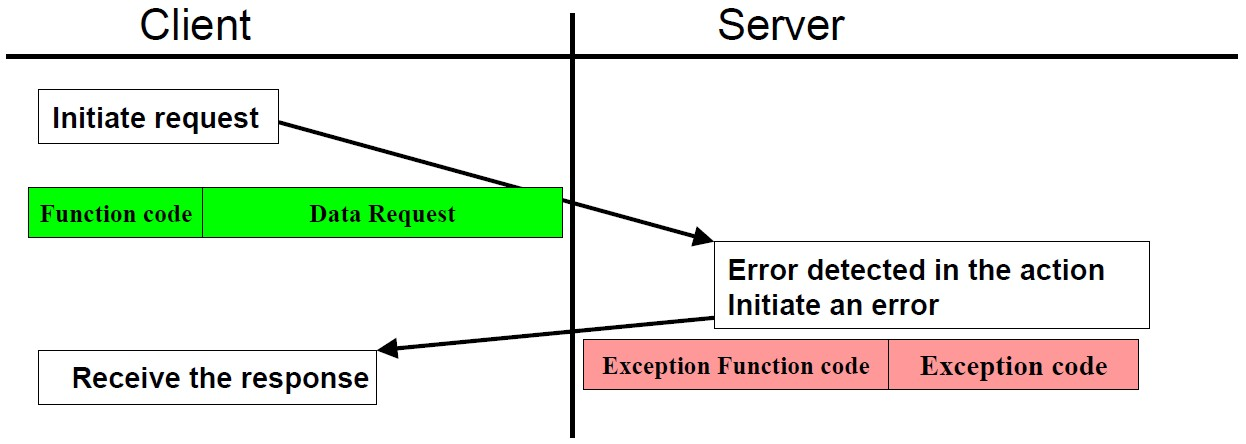
\includegraphics[width=14cm]{BilderAllgemein/ClientServerException.jpg}\medskip
 	\caption{Exception Antwort einer Modbus Transaktion \cite[S.4]{ModbusSpecification}}
 	\label{fig:FehlerTransaktion}
\end{figure}


\subsection{Modbus Datenmodell}
In Tabelle \ref{tab:modbusDataModel} werden die 4 unterschiedlichen Objekttypen, die von Modbus unterstützt werden, dargestellt. Daraus ist ersichtlich, dass eine Adresse auf nur 1 Bit oder auf einen 16 bit langen Bereich verweisen kann. Für die Adresse wird ein Wort (2 Byte) verwendet. Das bedeutet, es können von jedem Objekttyp 65536 Einträge am Modbus Server adressiert werden. Die Modbusadresse verweist auf den Wert, der von der Applikation, auf der der Server läuft, im Speicher gehalten wird. Abhängig vom Objekttyp kann der Wert von der Applikation bzw. vom Modbus Server gelesen oder gelesen/beschrieben werden.
Daraus ergeben sich unterschiedliche Möglichkeiten, das Modbus Datenmodell aufzubauen. Es kann ein Datenmodell aufgebaut werden, in dem sich alle Objekttypen einen Bereich teilen. Die zweite Möglichkeit ist, dass ein Modell aufgebaut wird, bei dem jeder Objekttyp auf einen separaten Datenbereich zeigt. Welche Daten hinter den Registeradressen stehen, ist der Applikation, welche auf dem Modbusserver läuft, überlassen \cite{ModbusSpecification, wilamowski2011industrial}. 

\begin{table}[h]
\centering
\begin{tabular}{|l|l|l|l|}
\hline
Register         & Länge  & Funktion & Beschreibung                                                                                     \\ \hline
Discrete Input   & 1 bit  & read     & \begin{tabular}[c]{@{}l@{}}Digitaleingang, welcher vom\\ Client gelesen wird\end{tabular}        \\ \hline
Coil             & 1 bit  & read/write      & \begin{tabular}[c]{@{}l@{}}Digitalausgang, welcher vom\\ Client beschrieben wird\end{tabular}    \\ \hline
Input Register   & 16 bit & read     & \begin{tabular}[c]{@{}l@{}}Bereich für die Darstellung\\ eines Werts für den Client\end{tabular} \\ \hline
Holding Register & 16 bit & read/write      & \begin{tabular}[c]{@{}l@{}}Bereich für das Schreiben\\ eines Werts an den Server\end{tabular}    \\ \hline
\end{tabular}
\caption{Modbus Datenmodell \cite{ModbusSpecification}}
\label{tab:modbusDataModel}
\end{table}
\clearpage

Abbildung \ref{fig:ModbusAddressModel} zeigt schematisch den Aufbau eines Modbus Geräts. Links ist die Applikation (\textit{Device application}), welche am Gerät läuft, dargestellt. Die grauen Felder sollen den Speicher der Anwendung darstellen. Abhängig vom Objekttyp werden die Werte im Speicher von der Applikation und vom Modbus Server gelesen und geschrieben. In der Mitte des Bildes ist das Modbus Datenmodell mit den Registeradressen dargestellt, welche auf den gemeinsamen Speicher zeigen. Rechts sind die Modbus Transaktionen dargestellt, die Daten aus dem Gerät, über die Register, lesen bzw. schreiben können \cite{ModbusSpecification}.

\begin{figure}[h]
	\centering
	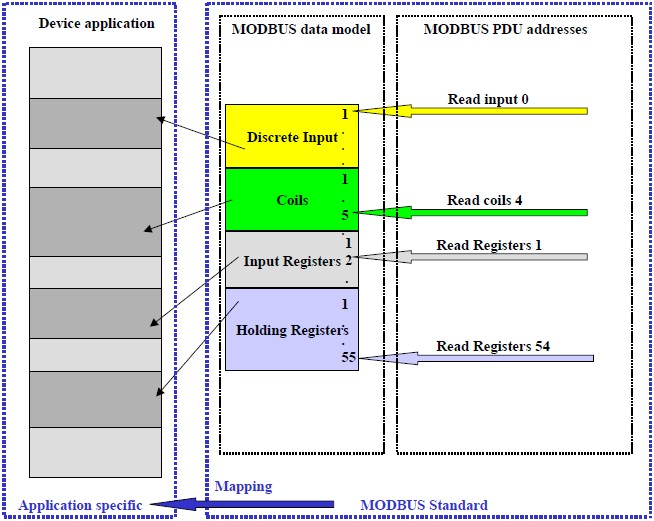
\includegraphics[width=14cm]{BilderAllgemein/ModbusAddressModel.jpg}\medskip
 	\caption{Modbus Adressmodell \cite[S.8]{ModbusSpecification}}
 	\label{fig:ModbusAddressModel}
\end{figure}
\clearpage

\subsection{Funktionscodes} 
\label{sec:Funktionscodes}
In diesem Abschnitt werden die zwei wichtigsten Funktionscodes, welche für die Implementierung benötigt werden beschrieben. Für diese werden nur Holding Register benötig. Deshalb werden hier nur die Funktionscodes behandelt, mit denen Holding Register beschrieben oder gelesen werden können \upshape\cite{SunspecInformationModelSpecification}.

\subsubsection{Lese Holding Registers}
\label{sec:LeseHoldingRegisters}
Bei der Verwendung des Funktionscode 0x03 wird ein zusammenhängender Block an \textit{Holding Register} gelesen. Wie Tabelle \ref{tab:ReqHoldingRegisters} zeigt, müssen in der PDU die Startadresse und die Anzahl an zu lesenden Registern übergeben werden. Ist die Transaktion erfolgreich am Server, dann wird derselbe Funktionscode zurückgesendet. In der PDU wird im ersten Byte die Anzahl an Werten zurückgegeben. Im übrigen Datenbereich befinden sich die Werte, auf welche die Register des Servers zeigen. Dies ist allgemein in Tabelle \ref{tab:RespHoldingRegisters} dargestellt. Tabelle \ref{tab:RespHoldingRegistersException} zeigt die Antwort bei einem Fehler der Transaktion am Server. Tritt ein solcher Fehler auf, dann wird zum Funktionscode 0x80 addiert. Dieser neue Funktionscode wird zurück an den Client gesendet. Weiters wird in das Datenfeld der Exceptioncode geschrieben. Dieser gibt Aufschluss über die Art des Fehlers und kann vom Client ausgewertet werden \upshape \cite{ModbusSpecification}. 


    \begin{table}[h]
		\centering
		\begin{tabular}{|l|l|l|}
			\hline
			Funktionscode       & 1 Byte & 0x03              \\ \hline
			Startadresse        & 2 Byte & 0x0000 ... 0xFFFF \\ \hline
			Anzahl der Register & 2 Byte & 1 ... 125         \\ \hline
		\end{tabular}
		\caption{Anforderung Lese Holding Registers \cite{ModbusSpecification}}
		\label{tab:ReqHoldingRegisters}
	\end{table}
	\begin{table}[h]
		\centering
		\begin{tabular}{|l|l|l|}
			\hline
			Funktionscode       & 1 Byte      & 0x03   \\ \hline
			Anzahl an Bytes		& 1 Byte      & 2 x N* \\ \hline
			Register Wert       & N* x 2 Byte &        \\ \hline
		\end{tabular}
		\caption{Antwort Lese Holding Registers wenn erfolgreich \cite{ModbusSpecification}}
		\label{tab:RespHoldingRegisters}
	\end{table}
	\begin{table}[h]
		\centering
		\begin{tabular}{|l|l|l|}
			\hline
			Fehler code    & 1 Byte & 0x83           \\ \hline
			Exception code & 1 Byte & 01, 02, 03, 04 \\ \hline
		\end{tabular}
		\caption{Antwort Lese Holding Registers wenn Fehler \cite{ModbusSpecification}}
		\label{tab:RespHoldingRegistersException}
	\end{table}
\clearpage

\subsubsection{Schreibe Multiple Registers}
\label{sec:SchreibeMultipleRegister}
Bei der Verwendung des Funktionscodes 0x10 können mehrere Werte in einem zusammenhängenden Block von Holding Registern geschrieben werden. Byte 0 der PDU ist der Funktionscode. In der PDU müssen das erste und zweite Byte die Registeradresse sein. Byte drei und vier sind die Anzahl der Register, welche beschrieben werden sollen. Byte fünf ist die Anzahl an zu schreibenden Bytes. Abhängig davon wie viele Werte geschrieben werden müssen, ist die restliche Anzahl an nicht verwendeten Bytes in der PDU für die Werte die geschrieben werden sollen vorgesehen. Dies zeigt Tabelle \ref{tab:ReqWriteMultipleRegisters}. Tabelle \ref{tab:RespWriteMultipleRegisters} stellt den generellen Aufbau der PDU dar, wenn das Schreiben der Register erfolgreich war. Hier wird wieder der selbe Funktionscode vom Server zurückgesendet. Weiters steht in den Daten die Offset Registeradresse, ab der die Daten an den Server geschrieben wurden, sowie die Anzahl an Registern. Bei einem Fehler wird der Aufbau der Antwort vom Servers gleich, wie schon in Abschnitt \ref{sec:LeseHoldingRegisters} generiert. Spezifisch für die Funktion Schreibe Multiple Registers ist dies in Tabelle \ref{tab:RespWriteMultipleRegistersException} dargestellt \upshape \cite{ModbusSpecification}.

    \begin{table}[h]
		\centering
		\begin{tabular}{|l|l|l|}
			\hline
			Funktionscode       & 1 Byte & 0x10              \\ \hline
			Startadresse	    & 2 Byte & 0x0000 ... 0xFFFF \\ \hline
			Anzahl der Register & 2 Byte & 1 ... 125         \\ \hline
			Anzahl an Bytes		& 1 Byte & 2 x N* 			 \\ \hline
			Register Werte      & N* x 2 Byte &        		 \\ \hline
		\end{tabular}
		\caption{Anforderung Schreibe Multiple Registers \cite{ModbusSpecification}}
		\label{tab:ReqWriteMultipleRegisters}
	\end{table}
	\begin{table}[h]
		\centering
		\begin{tabular}{|l|l|l|}
			\hline
			Funktionscode       & 1 Byte      & 0x10   			  \\ \hline
			Startadresse	    & 2 Byte 	  & 0x0000 ... 0xFFFF \\ \hline
			Anzahl der Register & 2 Byte      & 0x0000 ... 0xFFFF \\ \hline
		\end{tabular}
		\caption{Antwort Schreibe Multiple Registers wenn erfolgreich \cite{ModbusSpecification}}
		\label{tab:RespWriteMultipleRegisters}
	\end{table}
	\begin{table}[h]
		\centering
		\begin{tabular}{|l|l|l|}
			\hline
			Fehler code    & 1 Byte & 0x90           \\ \hline
			Exception code & 1 Byte & 01, 02, 03, 04 \\ \hline
		\end{tabular}
		\caption{Antwort Schreibe Multiple Registers wenn Fehler \cite{ModbusSpecification}}
		\label{tab:RespWriteMultipleRegistersException}
	\end{table}
\clearpage

\subsection{ModBus TCP/IP}

Bei Modbus TCP/IP oder kurz  Modbus TCP sind Server und Client über ein Ethernet TCP/IP Netzwerk miteinander verbunden. Die PDU des Modbus Protokoll wurde bereits im Abschnitt \ref{sec:Protokollaufbau} beschrieben. Dieses Kapitel behandelt die ADU bei der Verwendung des TCP. Anhand von Abbildung \ref{fig:ModbusFrame} ist bereits der Aufbau eines Modbus RTU Frames erklärt worden. Bei diesem besteht die ADU aus \textit{Slave ID} und \acs {CRC}. Diese werden bei einem seriellen Netzwerk verglichen mit dem OSI Schichtmodell an der untersten Schicht hinzugefügt bzw. implementiert. Bei der Verwendung von TCP kommt zur Modbus PDU der \ac {MBAP} Header hinzu. In diesem ist nun die \textit{Slave ID} welche bei TCP \textit{Unit ID} genannt wird, enthalten. Bild \ref{fig:ModbusADUCompare} stellt auch die weiteren Felder des MBAP Headers dar. Diese bestehen aus der \textit{Transaction ID}, welche vom Client bei einer Transaktion vergeben wird, weiters die \textit{Protocol ID}, welche für Modbus immer 0 ist und das Feld \textit{Lenght}, das die Anzahl der darauffolgenden Bytes angibt. CRC wird nicht in die TCP ADU übernommen. Diese Funktion erledigen die darunterliegenden Protokolle \cite{ModbusTCPImplementation, ModbusRTUImplementation, marshall2005industrial}.

\begin{figure}[h]
	\centering
	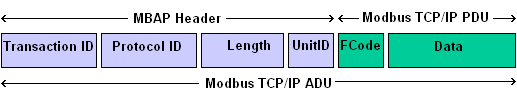
\includegraphics[width=14cm]{BilderAllgemein/ModbusAduPdu.png}\medskip
 	\caption{Modbus ADU Vergleich \cite{SimplyModbus}}
 	\label{fig:ModbusADUCompare}
\end{figure}
\newpage

Abbildung \ref{fig:ModbusEncapsulation} zeigt prinzipiell, wie die Modbus TCP ADU in den TCP Frame eingepackt wird. Auch wird dargestellt, dass Ethernet nun den \textit{Error Check} durchführt. Für Modbus TCP ist der Port 502 reserviert \upshape \cite{ModbusTCPImplementation}.

\begin{figure}[h]
	\centering
	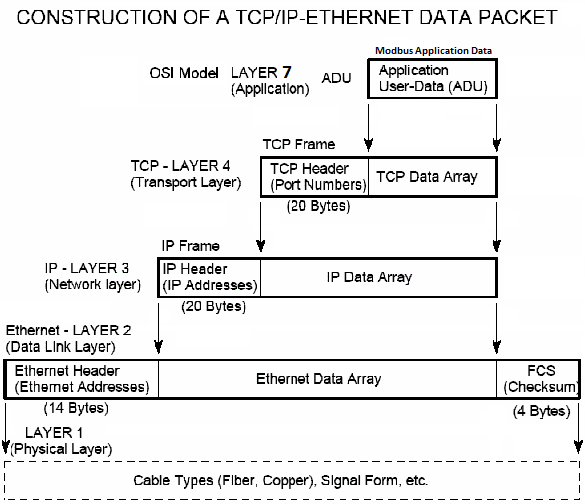
\includegraphics[width=14cm]{BilderAllgemein/ModbusEncapsulation.png}\medskip
 	\caption{Modbus Encapsulation bei TCP/IP \upshape \cite{SimplyModbus}}
 	\label{fig:ModbusEncapsulation}
\end{figure}

\newpage
Wie schon in Abschnitt \ref{sec:Protokollaufbau} beschrieben, ist für die Slave ID nur ein Byte reserviert. In einem seriellen Netzwerk können so theoretisch 256 Server adressiert werden. 0 ist die Broadcast Adresse. Die Adressen 248 - 255 sind reserviert. Daraus ergeben sich gültige Adressen von 1 - 247 für die Server in einem seriellen Netzwerk. Ein Modbus TCP Gerät kann somit auch nur auf 247 Server routen. Abbildung \ref{fig:ModbusTCPArchitecture} zeigt, wie ein TCP Gerät als Gateway zu einem seriellen Netzwerk fungiert. In TCP/IP Netzwerken ist jedoch die Anzahl an Modbus Servern, die adressiert werden können, nicht mehr von der Slave ID alleine abhängig. Jedes Modbus Gerät in diesem Netzwerk hat eine IP Adresse und somit ist die Anzahl abhängig von den möglichen IP-Adressen in einem Netzwerk \cite{ModbusTCPImplementation, wilamowski2011industrial}.

\begin{figure}[h]
	\centering
	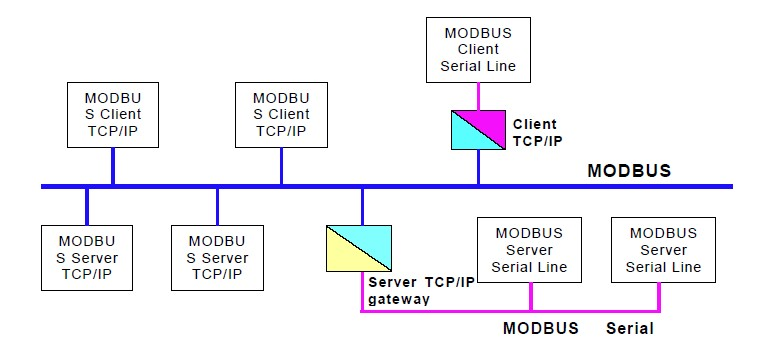
\includegraphics[width=14cm]{BilderAllgemein/ModbusTCPArchitecture.jpg}\medskip
 	\caption{Modbus TCP/IP Kommunikations-Übersicht \upshape \cite[S.4]{ModbusTCPImplementation}}
 	\label{fig:ModbusTCPArchitecture}
\end{figure}
\vspace{10cm}
\clearpage

\section{SunSpec}

\subsection{Übersicht}
Die SunSpec Alliance hat es sich zur Aufgabe gemacht, einen de facto Standard zu entwickeln, um für erneuerbare Energiequellen eine einheitliche Schnittstelle zu schaffen. Ziel ist es dabei durch, den einheitlichen Standard die Kosten für die Errichtung neuer Anlagen oder auch die Implementierung neuer Geräte in ein bestehendes System zu senken. Unabhängig vom Hersteller des Modells soll auf Geräte wie Wechselrichter, Stromzähler, Panels usw. einheitlich zugegriffen werden können \upshape \cite{SunspecOverview}.

\subsection{SunSpec Informationsmodell}
\label{sec:SunsSpecInformationsmodell}
Aufgabe des Informationsmodells ist es, die Datenpunkte eines Geräts auf das verwendete Kommunikationsprotokoll zu abzubilden. Bei der Verwendung von Modbus TCP werden die Datenpunkte eines Gerätes eindeutig auf Registeradressen des Modbus Protokolls abgebildet. Hat der Client dasselbe Informationsmodell hinterlegt, kann dieser die Daten, welche in den Registern bereitgestellt werden wieder auf für die Applikation sinnvolle Daten zurückführen. Für ein gültiges SunSpec Gerät müssen Informationsmodelle zu einer Gerätebeschreibung strukturiert werden.

Es gibt 4 Typen von Informationsmodellen. Diese heißen folgendermaßen:
\begin{itemize}
    \item Common Model
	\item Standard Model(s)
	\item Vendor Model(s)
	\item End Model
\end{itemize}

Es werden mindestens 3 Informationsmodelle für eine Gerätebeschreibung benötigt. Dazu gehören das Common Model am Beginn und das End Model am Ende der Beschreibung, dazwischen muss sich mindestens ein Standard Model oder Vendor Model befinden. Das erste Register eines Informationsmodells verweist immer auf eine eindeutige ID. Im zweiten Register befindet sich die Länge des Modells. Das End Model markiert das Ende des SunSpec Gerätes. Dadurch kann ein Client durch alle Register iterieren und abhängig von den für ihn gültigen IDs die Daten nutzen \cite{SunspecInformationModelSpecification}.

\subsection{SunSpec Datentypen}
Modbus stellt wie bereits beschrieben nur 1 bit oder 16 bit lange Datentypen zur Verfügung. Für die Datenpunkte der SunSpec Implementierung werden aber Datentypen benötigt die größer als 2 Byte sind. Dieses Kapitel gibt eine Übersicht der verwendeten Datentypen. Diese sind wie folgt:

\begin{itemize}
    \item int: Integer Vorzeichenbehaftet
    \item uint: Integer Vorzeichenlos
    \item pad: Padding Feld, um ein Informationsmodell mit Leerdaten aufzufüllen
    \item acc: wird für Daten verwendet die akkumuliert werden wie z.B. Energieverbrauch.
    \item enum: Aufzählungstyp, wird verwendet für Status
    \item bitfield: Eine Zusammenfassung von bits.
    \item string: Zeichenkette
    \item ip: Datentyp für eine IP-Adresse
\end{itemize}

Ganzzahlige Datentypen verwenden gleich wie Modbus die Big-Endian Byte Reihenfolge.

Eine Aufzählung der Datentypen und deren Speicherbelegung.
\begin{itemize}
    \item Integer
    \newline Ein 16 bit Integer benötigt genau ein Modbus Register. Dies soll Tabelle \ref{tab:16bitInteger} zeigen. Weiters soll diese Tabelle als Beispiel für größere Ganzzahlen wie 32, 64 und 128 bit Integer dienen. Der Aufbau ist bei diese Datentypen derselbe, nur dass dementsprechend mehr zusammenhängende Register benötigt werden.
    
    \begin{table}[h]
		\centering
		\begin{tabular}{|l|l|l|l|l|l|l|l|l|l|l|l|l|l|l|l|l|}
			\hline
			MB Register & \multicolumn{16}{l|}{1}                                             \\ \hline
			Byte            & \multicolumn{8}{l|}{0}              & \multicolumn{8}{l|}{1}        \\ \hline
			Bits            & 15 & 14 & 13 & 12 & 11 & 10 & 9 & 8 & 7 & 6 & 5 & 4 & 3 & 2 & 1 & 0 \\ \hline
		\end{tabular}
		\caption{16 bit Integer \cite[S.14]{SunspecInformationModelSpecification}}
		\label{tab:16bitInteger}
	\end{table}
	
\clearpage
    \item String
    \newline String plus die Längenangabe definiert die Anzahl an Zeichen. Tabelle \ref{tab:String} soll dies am Beispiel von einem SunSpec \textit{string16} zeigen. Die Registeranzahl für einen String wird folgendermaßen berechnet. Zuerst wird die Anzahl der Zeichen des Strings durch zwei dividiert. Das Ergebnis dieser Division aufgerundet auf die nächsthöhere Ganzzahl ergibt die Anzahl der benötigten Register. Mit NULL (ASCII 0x0) kann ein String frühzeitig abgeschlossen werden.

	\begin{table}[h]
		\centering
		\begin{tabular}{|l|l|l|l|l|l|l|l|l|l|l|l|l|l|l|l|l|}
			\hline
			MB Register & \multicolumn{2}{l|}{1} & \multicolumn{2}{l|}{2} & \multicolumn{2}{l|}{3} & \multicolumn{2}{l|}{4} & \multicolumn{2}{l|}{5} & \multicolumn{2}{l|}{6} & \multicolumn{2}{l|}{7} & \multicolumn{2}{l|}{8} \\ \hline
			Byte        & 0          & 1         & 2          & 3         & 4          & 5         & 6         & 7          & 8          & 9         & 10         & 11        & 12         & 13        & 14        & 15         \\ \hline
			Character   & E          & X         & A          & M         & P          & L         & E         & spc        & S          & T         & R          & I         & N          & G         & !         & NULL       \\ \hline
		\end{tabular}
		\caption{String \cite[S.15]{SunspecInformationModelSpecification}}
		\label{tab:String}
	\end{table}

    \item Gleitkommadarstellung
    \newline Eine Gleitkommazahl wird 32 bit codiert nach IEEE 754. Tabelle \ref{tab:float} zeigt, welche Registerbits für welche Felder der Gleitkommazahl verwendet werden.
    
    \begin{table}[h]
		\centering
		\begin{tabular}{|l|l|l|l|l|l|}
			\hline
			MB Register & \multicolumn{3}{l|}{1}             & \multicolumn{2}{l|}{2} \\ \hline
			Byte        & \multicolumn{2}{l|}{0} & 1         & 2          & 3         \\ \hline
			Bits        & 31      & 30 ... 24    & 23 ... 16 & 15 ... 8   & 7 ... 0   \\ \hline
			IEEE 754    & Vorzeichen    & Exponent     & \multicolumn{3}{l|}{Mantisse}      \\ \hline
		\end{tabular}
		\caption{Float \cite[S.16]{SunspecInformationModelSpecification}}
		\label{tab:float}
	\end{table}

	\item Skalierungsfaktoren
    \newline Wenn keine Gleitkommazahlen in der Applikation des Clients verwendet werden können, ist es möglich, die Datenpunkte als Integer Werte darzustellen. Der Skalierungsfaktor schiebt dabei das Komma um n Stellen nach links oder rechts. Der Wertebereich von n umfasst -10 bis 10. Das am Server verwendete Informationsmodell definiert, ob Gleitkommazahlen oder Ganzzahlen mit Skalierungsfaktoren verwendet werden \upshape \cite{SunspecInformationModelSpecification}.

\end{itemize}
\clearpage

\subsection{Register Mapping}

Bei der Verwendung von Modbus und SunSpec befindet sich in der Basis Registeradresse die 32bit lange SunS ID mit dem Wert 0x53756e53. Das Basis Register muss immer diesen Wert zurückgeben. Wird dieser Wert nicht zurückgegeben, dann muss dieser in einem der alternativen Basis Register stehen. Ist dies nicht der Fall, dann handelt es sich nicht um ein SunSpec Gerät. Nach den 2 Registern für die SunS ID muss im folgenden Register die ID für das Common Model stehen. Der restliche Teil der Register ist so aufgebaut, wie im Unterkapitel \ref{sec:SunsSpecInformationsmodell} beschrieben \upshape \cite{SunspecInformationModelSpecification}.

SunSpec gibt folgende Basis Register vor:
\begin{itemize}
    \item Basis Register: 40001
    \item Alternatives Register: 50001
    \item Alternatives Register: 00001

\end{itemize}
\clearpage

